\documentclass[11pt,letterpaper]{article}
\usepackage[margin=0.85in]{geometry}
\usepackage[T1]{fontenc}
\usepackage{times,amsmath,amssymb,graphicx,booktabs,array,longtable}
\usepackage{caption,xcolor,listings,enumitem,url}
\usepackage[numbers,sort&compress]{natbib}
\usepackage[colorlinks=true,linkcolor=blue!45!black,citecolor=blue!45!black,urlcolor=blue!45!black]{hyperref}
\setlength{\parindent}{0pt}
\setlength{\parskip}{5pt}
\setlength{\textfloatsep}{12pt}
\setlength{\floatsep}{10pt}
\setcounter{tocdepth}{1}
\numberwithin{equation}{section}
\numberwithin{figure}{section}
\numberwithin{table}{section}
\newcommand{\neval}{\texttt{NOT\_EVALUABLE}}
\newcommand{\code}[1]{\texttt{#1}}
\newcommand{\sourcefile}[1]{\texttt{\detokenize{#1}}}
\lstset{basicstyle=\ttfamily\fontsize{9}{11}\selectfont,breaklines=true,columns=fullflexible,keepspaces=true,showstringspaces=false,frame=single,framerule=.2pt,rulecolor=\color{gray},xleftmargin=2pt,xrightmargin=2pt}
\captionsetup{font=small,labelfont=bf}
\setlist{nosep,leftmargin=1.5em}
\hypersetup{pdftitle={TopoWorld-Eval: Supplementary Technical Report},pdfauthor={Jincheng Li; Yuxuan Li},pdfsubject={Public supplementary technical report}}
\begin{document}
\begin{titlepage}
\centering
\vspace*{1.15in}
{\LARGE\bfseries TopoWorld-Eval\par}
\vspace{.25in}
{\Large From Spatial Answers to Coherent, Grounded,\par and Revisable Executable Worlds\par}
\vspace{.4in}
{\large Supplementary Technical Report\par}
\vspace{.2in}
Jincheng Li\qquad Yuxuan Li\par
\vspace{.6in}
\begin{minipage}{.88\textwidth}
This report provides the dataset qualification, exact task conditions, executable representation, evaluator audit, full results, and reproducibility procedure behind the main paper. It separates correct relation answers, valid world construction, material coherence, image grounding, and evidence revision.

The static study contains 14 physical buildings and 42 drawing pages. Eight fixed Codex product configurations contribute 624 static task allocations and 64 revision stages. A tool-free Qwen API condition contributes 42 further allocations. Repeated conditions on the same buildings remain identifiable throughout.

All reported primary scores use the retained first outputs and the declared evaluator versions. The accompanying package supports deterministic rescoring. It makes no model request. Historical pilots and software fixtures are marked separately from the primary study.
\end{minipage}
\vfill
Public technical report release: 6 November 2026\par
Frozen primary evaluator: 2.2.1\par
\end{titlepage}
\tableofcontents
\vspace{.3in}
\textbf{Reading guide.} For source qualification, start with Appendix~\ref{app:A}. For exact inputs, use Appendix~\ref{app:B}. Appendices~\ref{app:C}--\ref{app:D} explain what the representation and checker actually compute. Appendices~\ref{app:E}--\ref{app:H} separate static GPT results, Qwen, grounding, and revisions. Appendix~\ref{app:I} shows retained geometric examples. Appendix~\ref{app:J} gives the statistics and replay procedure.

\textbf{Terminology.} R is independent relation answering; A is image-conditioned world construction; B adds correct determinate relation values. These are the primary R/A/B conditions, not the older B0/B1 labels. The historical A/B/C/D pilot uses a different design and appears only in Appendix~\ref{app:H}. A product model alias identifies a recorded Codex setting, not a verified immutable neural checkpoint.

\appendix
\clearpage\section{Dataset and Reference Qualification}\label{app:A}
\subsection{Scientific target and sampling unit}
TopoWorld-Eval asks whether an AI can maintain one grounded spatial world across views, tasks, and later evidence changes. A successful response should refer to the same physical instances across drawings, realize the supported spatial relations in executable geometry, avoid represented material conflicts, and revise evidence-dependent claims when a source changes. These requirements are related, but success on one does not establish success on the others.

The primary static material consists of public architectural drawings for 14 physical buildings. Twelve buildings occur in both the original semantic-locator condition v1 and its neutral-locator control N2. Two further complex-staircase buildings occur in CS1. Thus v1 plus N2 does not provide 24 independent buildings. The repeated conditions instead provide controlled comparisons on the same visual material. Likewise, eight configurations and several queries per building increase the number of observations without increasing the number of sampled buildings.

The material supports bounded target-fragment evaluation. It does not require reconstruction of every wall or opening in a complete building. Targets concentrate on floor relationships, doors and windows, staircase endpoints, and identity across drawing views. The sample includes schools, houses, civic buildings, missions, and institutional quarters. It was assembled for these structural questions rather than drawn as a random sample of all architecture. The empirical conclusions therefore concern the observed buildings and task conditions.

\subsection{Building and drawing inventory}
Table~\ref{tab:A-catalogue} identifies all buildings. The 12 N2 cases contain 35 pages, rendered at a 3,200-pixel long side. CS1 adds seven pages at a 3,000-pixel long side. Original source identifiers, public page URLs, image dimensions, and SHA-256 values are preserved in the package catalogue. View identifiers were shuffled in N2; the catalogue retains the mapping to the source page.

\begin{table}[htbp]\centering\small
\begin{tabular}{p{.20\linewidth}p{.57\linewidth}r}
\toprule Case & Building / source collection & Pages\\\midrule
A01 & Octagon House, Washington DC; HABS DC-25 & 3\\
A02 & Drayton Hall, South Carolina; HABS SC-377 & 3\\
A06 & Octagon House, Watertown; HABS WI-135 & 3\\
B01 & Westside School, Las Vegas; NV0473 & 3\\
B02 & Madison County Courthouse, Virginia City; MT0028 & 3\\
B03 & San Xavier del Bac Mission, Tucson; AZ0061 & 3\\
B04 & Mission San Luis Obispo Monastery; CA0801 & 3\\
B05 & Mission Frame House, Honolulu; HI0032 & 3\\
B06 & William Scarborough House, Savannah; GA0030 & 3\\
C01 & Quarters No. 211, San Juan; PR0070 & 3\\
C02 & Rock Schoolhouse, Fillmore; UT0027 & 2\\
C03 & Idaho City Schoolhouse; HABS ID-6 & 3\\\midrule
CS1--S01 & Lovell Health House; HABS CA-1936 & 3\\
CS1--S02 & Gamble House; HABS CA-1981 & 4\\\bottomrule
\end{tabular}
\caption{The 14 physical buildings and 42 whole-page drawings. Short case IDs are expanded to their stable package IDs in the catalogue. v1 and N2 reuse the first 12 buildings.}\label{tab:A-catalogue}
\end{table}

Public availability and a source citation do not by themselves establish a blanket redistribution license for every archival item. The package retains the Library of Congress source and rights information where supplied. Private Loft photographs and account information are excluded. Historical Loft examples in the casebook use reconstructed coordinates and diagnostic diagrams, not private image files.

\subsection{Reference obligations and evidence isolation}
The fixed list contains 96 relation obligations: 95 determinate values and one explicitly unresolved identity. N2 contributes 75 determinate values and one unknown; CS1 contributes 20 determinate values. Across the 95 determinate obligations, 71 are TRUE and 24 are FALSE. The predicate distribution appears in Table~\ref{tab:A-predicates}. Queries are frozen obligations, not relations selected after seeing an output. Some require several pages; others concern multiple drawings on one sheet.

\begin{table}[htbp]\centering
\begin{tabular}{lr@{\qquad}lr}\toprule
Predicate & Count & Predicate & Count\\\midrule
\texttt{connected\_by} & 4 & \texttt{same\_floor} & 11\\
\texttt{above} & 14 & \texttt{window\_host} & 17\\
\texttt{identity\_assignment} & 23 & \texttt{door\_host} & 8\\
\texttt{disjoint} & 9 & \texttt{stair\_connects} & 10\\\bottomrule
\end{tabular}
\caption{All 96 obligations, including the one unresolved identity. Types are not equally frequent or equally difficult.}\label{tab:A-predicates}
\end{table}

Each reference record identifies the query, arguments, frozen value, source page, and supporting explanation. The audit also links approximate crops and target points for human review. These review crops are derivatives; they were not additional model inputs. The reference geometry is not a unique coordinate model. When several geometric completions can express the same supported relation, the benchmark allows them rather than requiring a hidden metric reconstruction.

The reference list and the model input are separate objects. R and A do not receive organizer relation answers. B deliberately receives the determinate relation values as a controlled input. It receives neither hidden reference coordinates nor the organizer's localization boxes. B therefore measures construction with relation assistance. It cannot be described as unaided image reconstruction.

Reference records retain their historical AI-assisted annotation metadata. Later, the author explicitly confirmed personally checking all 96 relations. The completion record preserves this statement without changing the frozen values. No separate per-item verdict file or second expert's review was supplied. Accordingly, the correct qualification is author-reviewed, AI-assisted reference construction. Inter-annotator agreement and independent expert certification have not been measured.

\subsection{How to inspect a reference}
A reviewer can start with a query row, open its listed public page, locate its target point, and then inspect the indicated source region. For an identity query, both observations must be checked. A repeated printed label can be a component type rather than a physical instance. For a staircase, the review must distinguish the whole assembly, a run, a landing, and a nearby space. The question must also refer to a supported granularity: the endpoint of a two-riser transition is not necessarily the endpoint of a complete multi-floor staircase.

The evidence table records what the drawing supports and what remains unknown. It does not infer a removed wall from an omitted drafting line, public access from physical contact, or physical identity from equal labels. If a source is a historical plan and another page represents a different state, matching image position is insufficient to assert that an opening is the same surviving object.

The single unresolved case is B04's cross-era identity. The selected pages do not establish whether the two observations are one persisting physical instance. UNKNOWN is the supported epistemic answer. A definite SAME answer is unsupported certainty; it is not necessarily a proven false statement about the actual building. This distinction matters when interpreting the low uncertainty score in Appendix~\ref{app:G}.

\begin{figure}[htbp]\centering
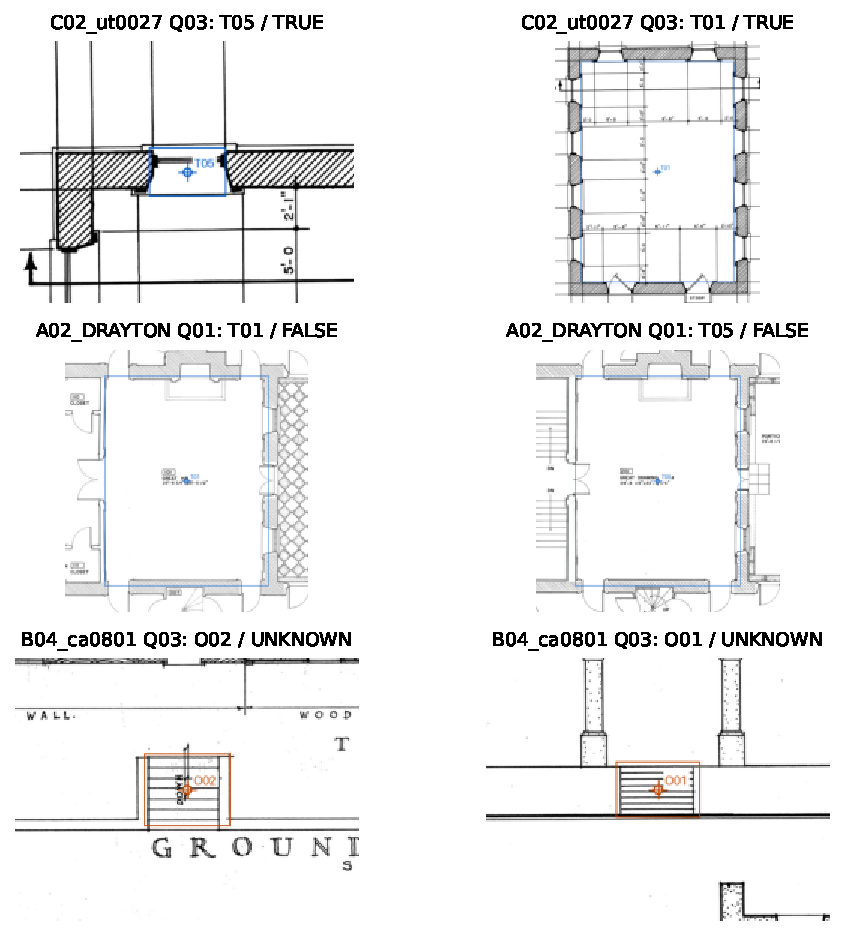
\includegraphics[width=.94\linewidth]{figures/reference_evidence.pdf}
\caption{Three source-to-reference examples: an opening incident to its classroom, two spaces on different floors, and a cross-era identity that remains unresolved. These organizer-review crops show the reference regions, not model boxes. Public page IDs and parent hashes are retained; the models received full assigned pages.}\label{fig:A-reference}
\end{figure}

\subsection{Controls on task difficulty and label imbalance}
N2 removes semantic identifiers such as named floors or room labels from organizer-provided target names. It replaces them with arbitrary T/O identifiers, shuffled V identifiers, point locators, and optional class hints. Text actually printed in an image remains available. The control therefore reduces organizer-supplied answer cues while retaining a feasible given-point localization task. It is not unprompted object discovery.

CS1 adds complex staircase cases and explicit granularity hints. These hints identify what assembly or local step transition is queried; they do not supply the answer or a correct coordinate model. CS1 also balances its determinate values, with ten TRUE and ten FALSE. It is a separate two-building challenge set, not an estimate of prevalence across all complex buildings.

For N2 alone, a constant TRUE predictor obtains 61/75, or 81.33\%. This simple diagnostic makes the label skew visible. It cannot construct a world, localize objects, or explain an identity. Still, it is a necessary reference when interpreting a high direct-answer percentage. Balanced CS1 and predicate-specific results help show which parts of the task exceed this shortcut.

The evaluation tasks were frozen before their respective model allocations. The study does not claim all drawings were unknown to model pretraining. The controls concern exposure through this experiment, not unverifiable historical training data. Future data collection should add independently qualified buildings and further uncertainty cases rather than treating more questions on the current drawings as new buildings.

\clearpage\section{Task Prompts, Inputs, and Execution Conditions}\label{app:B}
\subsection{Three independent static routes}
R independently answers a fixed relation list from the assigned drawings and target descriptions. A independently constructs an executable world from the same core evidence. Its answers are then read from the submitted world. B constructs a world with the additional correct determinate relation list. R is not used to initialize A, and A is not used to initialize B. The pairing unit is the same building, product configuration, and query, not an assumed shared hidden reasoning state.

This design distinguishes two questions. R versus A asks whether a configuration performs similarly when answering and constructing. A versus B asks whether correct relation input improves the construction. A lower A score does not prove that one particular generation internally knew a correct answer and lost it during serialization. A B failure shows that supplied relations were not successfully realized under the output contract; its cause can still be parsing, representation, geometry, identity, or localization.

\begin{table}[htbp]\centering\small
\begin{tabular}{p{.13\linewidth}p{.35\linewidth}p{.40\linewidth}}\toprule
Route & Allowed scientific evidence & Required output\\\midrule
R & Assigned pages, locators, fixed queries & Relation-answer JSON with source references\\
A & Same core evidence; world Schema and contract & One executable world; no direct answer table\\
B & A inputs plus correct determinate relation values & One executable world realizing the supplied relations\\\bottomrule
\end{tabular}
\caption{The primary routes. Neither model outputs nor organizer coordinates are passed across routes. Qwen R's additional generic Schema is an interface difference described in Appendix~\ref{app:F}.}\label{tab:B-routes}
\end{table}

\subsection{Exact prompts and a complete bounded example}
The release includes the saved prompt text for each route and condition. Paths are translated to package-relative paths in the portable copy. The scientific wording, query values, and image pixels are retained. Listings~\ref{lst:B-common}--\ref{lst:B-task} give the common N2 instruction and the complete compact Rock Schoolhouse task specification. The listings use portable formatting for readability; the saved text files are the exact wording record. A/B additionally receive the frozen Schema. The B relation supplement is separate from the task file and is included with the example.

\lstinputlisting[caption={N2 common scientific and execution instruction, shared by the example routes.},label={lst:B-common}]{examples/N2_COMMON.txt}

\subsection{Route-specific final instructions}
The common prompt ends with an assigned task identifier and one of the following instructions. These are transcribed from the saved N2 prompts. R's answer wrapper is fixed; geometry is not requested in R.
\begin{lstlisting}
R: Independently answer the fixed questions from these images.
Return one plain JSON object:
{"schema":"topoworld_relation_answers_v1","case_id":"C02_ut0027",
 "answers":[{"query_id":"...","value":"TRUE|FALSE|UNKNOWN|NOT_FOUND or numeric value",
 "evidence":[{"view_id":"...","description":"..."}]}]}.
Include every query once. Do not build a world.

A/B: Construct one executable world matching the supplied
topoworld_executable_v1 Schema and case_id. Include task_bindings
for every target role and observations for every requested anchor.
Return plain JSON, not a direct answer table.

A: Infer the target structure from the images and neutral task
locators. No correct relation table or previous output is supplied.

B: The given_correct_relations are independently source-checked
input. Realize these relations in actual geometry/identity
assignments, without access to reference coordinates.
\end{lstlisting}

\lstinputlisting[caption={Complete scientific task content for the two-page C02 example. Paths are relative; image hashes are retained in the machine-readable task. No reference answer is in this file.},label={lst:B-task}]{examples/C02_TASK_COMPACT.json}

\begin{figure}[htbp]\centering
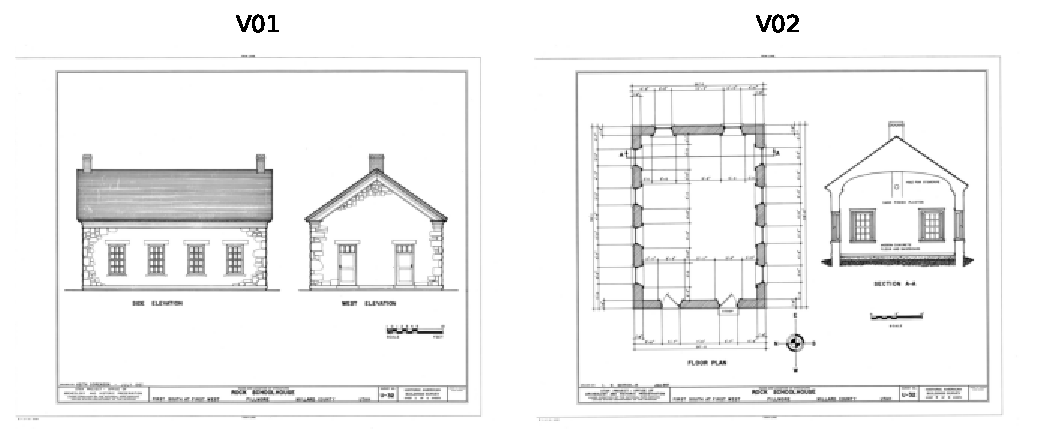
\includegraphics[width=.98\linewidth]{figures/C02_all_inputs.pdf}
\caption{All assigned image pages for the complete C02 example. The package includes these PNGs at their original task resolution. The printed overview is reduced for space and is not an alternative model input.}\label{fig:B-images}
\end{figure}

\paragraph{B-only relation supplement.} For this example, B additionally receives \texttt{Q01=TRUE}, \texttt{Q02=TRUE}, \texttt{Q03=TRUE}, \texttt{Q04=TRUE}, \texttt{Q05=TRUE}, \texttt{Q06=FALSE}. R and A do not receive this list. The full saved B task retains its machine-readable predicate arguments and values.

\subsection{Input conditions and output limits}
v1 supplies semantic target descriptions. N2 uses neutral IDs, point locators, and class hints; the input difference is intentional and must not be averaged away. CS1 uses neutral anchors with additional object-unit hints needed for complex multi-run and local-step questions. All three use the same bounded executable primitive family, but the content and difficulty of the tasks differ.

The construction contract limits the first output to 42,000 characters and 60 entities. It permits boxes, finite box unions, axis-aligned straight stair runs, and explicit unknown geometry. It asks for a shared coordinate frame, stable physical instances, observations with image boxes, target bindings, and evidence support. Unmeasured dimensions may be hypothetical completions. Such a completion must preserve supported relations, disclose uncertain parameters, and avoid claiming an exact recovered metric building.

The full Schema is supplied as a separate machine-readable file. It checks fields and types, not whether the building is correct. A syntactically valid response can fail the Schema; a Schema-valid response can still fail compilation or geometry. Conversely, an unknown geometry field can be valid while earning neither determinate readout nor required coverage.

\subsection{Codex context and tool boundary}
Each GPT task uses a fresh configuration-specific context derived from a READY-only seed, with the recorded product alias and \texttt{xhigh} setting. The seed carries the task rules, not a previous building answer. Each independent route receives its own job. The instructions allow assigned file/image reads, crops from the same pixels, and saving the first output. They prohibit other outputs, private references, external search, solver calls, evaluator feedback, and delegated solving.

This is an instruction-level boundary, not an operating-system filesystem sandbox. The audit retains observed departures. They include historical delegation-related missing outputs, one N2 computer-state request returning a locked/empty display, and CS1 access to an older public contract and a listing of temporary crop names. These events do not establish that hidden answers were read. They do prevent a claim that every run used an enforced identical sandbox. The primary results retain these allocations; sensitivity records identify their qualification.

Product names and effort settings are recorded as observed settings. The desktop interface does not provide a verified immutable neural checkpoint for each alias. We therefore report fixed Codex product configurations. We do not treat the eight configurations as eight independent provider families or equate their effort label with a measured floating-point budget.

\subsection{First-output policy and failed delivery}
The first complete response is saved before evaluation. The parser does not add a missing comma, deduplicate a key, fill a missing world, or infer an omitted endpoint. Empty, missing, malformed, oversized, and Schema-invalid outputs remain separate outcomes. A standard-path failure is not replaced using a better artifact discovered elsewhere. The independently retained wrong-location diagnostic remains outside the primary score.

All allocated determinate opportunities remain in the main denominator. A failed world can make several queries unevaluable; those are several missed obligations, not several independently established cognitive errors. A common-valid paired analysis is reported alongside the full denominator to isolate content differences after excluding delivery and format failures. It still includes geometric errors within valid outputs.

The task forbids an automatic generate--check--retry loop. The historical feedback pilot and evidence-revision stages have their own explicitly bounded designs. Their additional feedback is not retroactively allowed for the primary A/B routes. Repeating the deterministic scorer in the release changes no model response and is not a new attempt.

\clearpage\section{Executable Representation and Mathematical Semantics}
\label{app:C}

\subsection{A world, its observations, and its evidence}
The executable interface summarizes a model output as
\begin{equation}
W=(\mathcal O,\mathcal G,\alpha,\mathcal R,\mathcal P).
\end{equation}
Here $\mathcal O$ contains typed physical instances, assemblies, parts, and interfaces. $\mathcal G$ assigns supported geometric primitives and frames. The observation binding $\alpha$ maps image observations to declared instances. $\mathcal R$ contains typed declarations, including hosts, floors, and connections. $\mathcal P$ records sources, active status, and explicit evidence links. These fields organize an inspectable output; they do not define a learned representation or recover missing image evidence automatically.

The JSON contract also permits semantic types and depictions. A repeated window type code is therefore different from a physical window instance. The operational \code{identity\_assignment} reader compares the instance IDs assigned to two singleton observations. Equal IDs return true and unequal IDs return false for this \emph{assignment} measurement. The reference comparison determines whether that assignment is correct. This operation does not prove physical identity from pixels. The separate physical-identity predicates require compatible physical referents, and different IDs alone do not prove that two physical objects differ.

The same distinction applies to ownership. \code{owner} is descriptive text; \code{owner\_id} is an explicit identity field. The evaluator does not derive household identity from a room's position or from a descriptive string. Ownership, geometric connection, and permission to traverse remain separate. A source ID identifies evidence in the output ledger; its presence does not establish that the source supports the claim.

\subsection{Coordinates, units, and supported transformations}
World coordinates use two horizontal axes and an upward $z$ axis. Each executable box has finite bounds $a_j<b_j$ in all three dimensions. A local frame acts through
\begin{equation}
\begin{bmatrix}x'\\1\end{bmatrix}
=\begin{bmatrix}P&t\\0&1\end{bmatrix}
\begin{bmatrix}x\\1\end{bmatrix},
\qquad P\in\{0,\!\pm1\}^{3\times3},\quad P^\top P=I,
\end{equation}
with exactly one nonzero entry in each row and column of $P$. Thus the implemented transforms are signed axis permutations and translations. The compiler transforms all eight corners of a box. It does not silently approximate an arbitrary rotated solid with its bounding box. Straight stairs must remain compatible with the supported horizontal-run and upward-rise convention after transformation.

The evaluator accepts declared normalized, meter, foot, and inch units. Normalized coordinates do not establish metric dimensions. For recognized metric units, numerical tolerance is
\begin{equation}
\epsilon_u=10^{-6}/c_u,
\end{equation}
where $c_u$ is meters per declared unit. For normalized or unrecognized units, it is $10^{-6}$ in the declared coordinate unit. \code{apply\_evaluation\_policy} replaces a model-supplied arithmetic tolerance with this fixed policy and preserves the original declaration for audit. Adding a distant object therefore does not change local tolerance. This tolerance controls numerical comparisons, not a permitted construction error or a human clearance standard.

\subsection{Material, free regions, and openings}
The primitives are \code{box}, \code{box\_union}, \code{stair\_run}, and \code{unknown}. A box union denotes its actual union, not its enclosing box. Rooms and corridors are spatial regions. Walls, slabs, obstacles, and tread bodies occupy material. Their spatial overlap with a room is not itself a collision between two solids.

For a material host $h$, let $B_h$ be the union of its input boxes and let $V_h$ contain its compatible, explicitly registered opening volumes. The compiler computes
\begin{equation}
M_h=B_h\setminus\bigcup_{o\in V_h}B_o.
\label{eq:material-difference}
\end{equation}
Both \code{subtract\_union} and \code{contains\_union} operate on component boxes. Subtraction partitions a box into at most six remaining boxes per cut; the implementation caps the resulting representation at 4,096 boxes. A colored opening drawn over a complete wall does not remove material unless the host registers that opening. Conversely, the final wall interface can recognize an already cut host with an equivalent registered void (Appendix~\ref{app:D}).

The geometric predicates have different boundary conventions. \code{intersects} requires positive-volume material overlap above tolerance; mere touching does not satisfy it. \code{contains} checks that subtraction leaves no region. \code{projected\_crossing} checks nonempty overlap in a selected coordinate projection and may include boundary contact. It does not imply three-dimensional intersection. \code{above} and \code{below} require horizontal component overlap and vertical interval separation, rather than ordering entity centroids. Consequently, these names must be interpreted through their stated predicates, not through an informal drawing impression.

\subsection{Straight stairs and supported interfaces}
A straight run specifies lower endpoint $p_0$, upper endpoint $p_1$, width $w>0$, tread thickness $t>0$, and integer step count $2\le n\le128$. Exactly one horizontal coordinate changes. Let $r$ be that run coordinate, $a$ the constant transverse coordinate, and $\Delta z=z_1-z_0>0$. Writing each tread in $(r,a,z)$ coordinate order, for $i=0,\ldots,n-1$, define
\begin{align}
r_i&=r_0+(r_1-r_0)i/n,& z_i&=z_0+\Delta z(i+1)/n,\\
T_i&=[\min(r_i,r_{i+1}),\max(r_i,r_{i+1})]
\times[a-w/2,a+w/2]\times[z_i-t,z_i].
\end{align}
The compiler expands the run into $\bigcup_iT_i$. This geometry represents tread material, not a complete structural stair or an occupant swept volume.

Connection labels are obligations to check. \code{stair\_connection} tests the declared endpoint interfaces, landing hosts, endpoint heights, and supported floor-level connection to the named rooms. A room floor uses its exposed lower free-space boundary; a material landing uses its exposed top. The landing bridge must connect to a free room-floor component after subtracting material immediately above that level. Area overlap and positive-length edge contact can connect these floor charts; a corner-only contact cannot. Material ending at the floor can support the route without blocking it.

A compound stair declares finite straight runs and material landings. Its parent material must equal the union of the declared parts. The implemented assembly is a connected, nonbranching, acyclic chain with two external interfaces; nested or curved assemblies are outside this interface. The evaluator separately sweeps material over tread tops. A full-width occupied stripe extending above a tread is a definite obstruction. A side overlap without that condition can remain unresolved. The test does not establish body-height clearance or every possible walking trajectory.

\subsection{Door channels, window hosts, and route scope}
The final door reader evaluates connected opening components against retained wall material and the material-plus-void envelope. A through channel needs supported exterior ports on opposite wall faces and real material anchors. This rejects blind pockets and prevents a void extending beyond a wall from inventing a false wall-normal direction. A door must also reach the shared floor, have compatible opposite-side room incidence, and have its cut registered. A complete material blockage rejects the connection; a partial obstruction remains unresolved without a body profile. A window-host query verifies its typed wall, cut, boundary incidence, and declared room, without treating the window as a traversable door.

The derived route graph contains only interfaces whose connection checks return true. Graph reachability is therefore reachability through supported interfaces in the declared fragment. It does not prove that the whole building is navigable. Non-\code{ALL} permission scopes are not implemented, and \code{accessible} always returns \code{UNKNOWN}/\neval. Neither shared ownership nor a projected crossing adds a graph edge.

\subsection{Unknown geometry and alternative completions}
The broader scientific specification allows several worlds consistent with incomplete evidence. For active qualified evidence $E$, write
\begin{equation}
\mathcal S(E)=\{W:W\models E\},\qquad
q(E)=v\ \text{only if}\ \mathcal S(E)\ne\varnothing\ \text{and}\ \forall W\in\mathcal S(E),\ q(W)=v.
\end{equation}
This is an interpretation principle, not an implemented continuous-world enumeration algorithm. The current instrument reads one submitted world with bounded proof patterns. Explicit unknown geometry, absent required geometry, unresolved hosts, and unsupported operators remain unresolved. It does not choose a hidden favorable completion. Geometric parameters can be marked \code{EVIDENCE\_\allowbreak SUPPORTED}, \code{HYPOTHETICAL\_\allowbreak COMPLETION}, \code{MIXED}, or \code{UNKNOWN}; these declarations do not independently validate their evidence. Multiple different completions may pass the same qualified relational obligations.

\subsection{A complete runnable software example}
Listing~\ref{lst:stair-fixture} is a five-entity synthetic fixture, not a model prediction or a measured building. All dimensions are hypothetical. The two observation IDs deliberately bind to the same stair. The frozen 2.2.1 compiler accepts the complete listing. In a fresh replay, \code{stair\_connects} and \code{interface\_reachable} are true, \code{same\_floor(lo,hi)} is false, and \code{accessible} is unknown. These outputs demonstrate the distinction between a verified interface and human accessibility.

\begin{figure}[htbp]
\centering
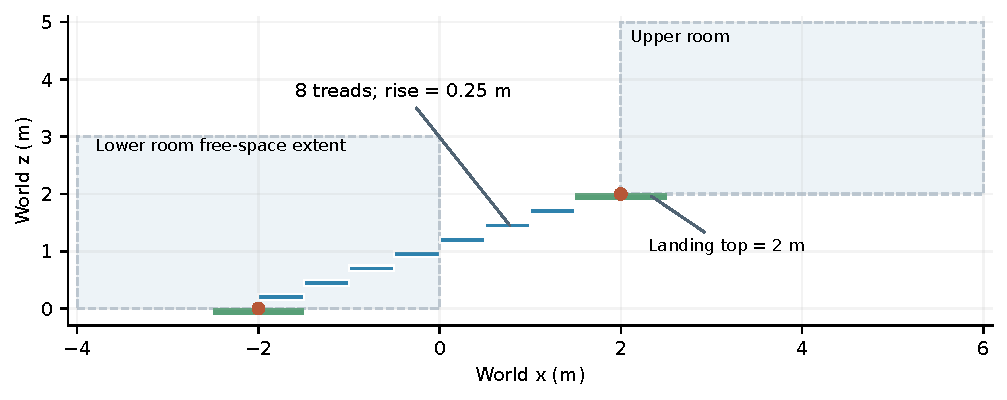
\includegraphics[width=.94\linewidth]{figures/verification/single_stair_fixture.pdf}
\caption{Compiled synthetic fixture in the $xz$ plane. Blue segments show the eight tread tops; green segments show material landings. Dashed boxes show room extents, not solid obstacles. The endpoint interfaces lie on the landing tops at $z=0$ and $z=2$ m. All plotted geometry comes from the same JSON listing.}
\label{fig:stair-fixture}
\end{figure}

\lstinputlisting[caption={Complete executable software fixture. Its observations are synthetic bookkeeping examples, with no image-grounding claim.},label={lst:stair-fixture},basicstyle=\ttfamily\fontsize{8}{9.5}\selectfont]{figures/verification/single_stair_listing.json}

The accompanying \sourcefile{figures/verification/verify_examples.py} checks this listing and four small door variants with byte-identical frozen code and Schema. The saved receipt contains five worlds and nine expected readouts. It is a software replay only; it adds no model trial or building sample.

\clearpage\section{Evaluator Architecture, Qualification, and Remaining Limits}
\label{app:D}

\subsection{From the retained response to independent readout}
The evaluation pipeline preserves the first delivered response, parses its JSON, checks the contract, compiles the geometry, and reads the registered queries. It then compares those readouts with the organizer's references. The geometric reader receives the submitted world and query specification, not the model's independent R answers or the hidden reference values. Rendering consumes the same world but does not rewrite it.

The organizer parser rejects duplicate JSON keys, nonfinite constants, and floating-point overflow. It records delivery and budget failures separately from physical verdicts. The frozen study permits 42,000 output characters and 60 entities. These experimental limits differ from the compiler's defensive limit of 256 entities and the component-operation cap of 4,096 boxes. A file can satisfy the JSON Schema yet fail a typed interface check. It can also compile while leaving a required geometric role unknown. Neither event should be silently repaired into success.

The scorer uses a disposable geometry worker with a 30-second wall limit. Its resource wrapper requests a 25-second soft CPU limit, a 30-second hard CPU limit, and a 1,536 MiB address-space limit where the operating system supports them. Worker errors and timeouts are execution outcomes, not false physical relations or proofs of inconsistency. Diagnostic lists may be compacted for logging, but this does not replace the scalar verdicts or drop failed task allocations from the accuracy denominator.

The code file retains earlier function definitions before later wrappers. The active 2.2.1 bindings, especially the final opening-host resolver and door reader, determine the results. Our implementation audit follows these bindings rather than describing the first function with a matching name. The frozen geometry file and Schema hashes are recorded in the reproducibility manifest and in the small software replay receipt.

\subsection{Five outputs with different meanings}
The instrument reports several measurements rather than treating every successful parse as a correct building. \textbf{Serialization validity} covers JSON and Schema. \textbf{Compilation} determines whether declared primitives can execute. \textbf{Query readout} returns a value, status, and a proof record containing the entities and checks used. \textbf{Registered geometry} covers the required geometric roles and their dependencies. \textbf{All-declared geometry} also checks additional structures generated by the model.

Registered scope starts from geometric target roles and follows supported references, including hosts, parts, connected rooms, endpoint interfaces, and openings. It does not automatically include every object mentioned by an identity observation. Thus a wrong observation-to-window assignment may affect the identity score without entering the registered geometric scope. Conversely, an extra internal staircase can fail the all-declared check while leaving registered target geometry unchanged. These two scopes answer different questions and remain separate in the tables.

A definite geometric contradiction produces \code{VIOLATION}. Relevant missing or unsupported information produces \neval. Missing or wrongly typed named door hosts produce an \code{UNKNOWN} readout with a \code{CONTRACT\_INVALID} status. They do not earn credit on a negative connectivity query. A determinate false connection with a valid host is different. \code{PASS\_REGISTERED\_GEOMETRY} and \code{PASS\_DECLARED\_FRAGMENT} apply only within their stated scopes. The instrument always leaves full-building success unevaluable because complete visual grounding and human-motion clearance are not established.

The all-declared verifier checks interfaces, material interactions, and supported declared relations. Aggregate stair parents are not counted a second time as independent collision solids when their parts already supply the material. For tread obstruction, the verifier also examines the union of relevant material. Splitting one full-width blocker into two half-width solids should not make the obstruction disappear. Declared relation agreement is retained separately from the registered geometric-coherence result, so a correct answer string cannot substitute for its supporting geometry.

\subsection{Saved software qualification}
Table~\ref{tab:evaluator-qualification} summarizes the qualification records associated with the frozen instrument. They are software checks, not additional model trials, independent buildings, or human annotations. We read the saved results and verified a small new fixture set for this report; we did not rerun the entire historical research pipeline.

\begin{table}[htbp]
\centering\small
\begin{tabular}{@{}p{.24\linewidth}p{.18\linewidth}p{.49\linewidth}@{}}
\toprule
Record & Saved result & Scope and interpretation\\
\midrule
2.2.1 unit qualification & 83 tests; 0 failures; 0 errors & Primitive arithmetic, interfaces, geometry counterexamples, and supported reader behavior.\\
Known-world checks & 8/8 Schema-valid and declared-fragment pass & Includes stairs, doors, windows, multiple hosts, a blocked door with a false readout, and an open passage.\\
Independent audit suite & 29/29 final checks pass & Separately constructed re-encodings and counterexamples; original frozen scores remain unchanged.\\
Blind-pocket grid & 0 unexpected accepts in 200 cases & Seeded synthetic diagnostic for the tested pocket family; not a universal false-positive bound.\\
Technical-report replay & 5 worlds; 9/9 expected readouts & Synthetic fixtures, including an equivalent pre-cut door and a malformed-host unknown.\\
\bottomrule
\end{tabular}
\caption{Qualification evidence for evaluator 2.2.1. Counts are not added to the model-study sample size. The independent audit is a separately constructed software suite, not an external building survey or expert certification.}
\label{tab:evaluator-qualification}
\end{table}

The independent audit retained its discovery history. An earlier candidate incorrectly accepted a blind pocket because a void overshooting the wall suggested an erroneous normal direction. The issue was reported and corrected before the final audit hash. The final 29 checks pass, and the subsequent 200-case grid has no unexpected acceptance in its tested family. Reporting this sequence is more informative than treating final qualification as evidence that every development version was correct.

\subsection{Why 2.2.1 changes the measured score}
Version 2.2.1 corrects four measurement problems: equivalent pre-cut wall material, connected stepped or splayed opening channels, void extensions below the active floor, and malformed hosts on negative queries. The wall reader reasons about retained material together with registered voids. Its active channel must have valid opposite exterior ports, material anchors, compatible room incidence, and floor contact. A subfloor extension cannot supply missing above-floor connectivity.

Figure~\ref{fig:opening-equivalence} gives a runnable example. The first encoding declares a solid wall and subtracts its registered door void. The second directly declares the retained wall union. The compiled material is mutually contained in both directions and has volume approximately $1.872\,\mathrm{m}^3$ in each case. Both door readouts are true. The blind-pocket control leaves material across the wall depth and reads false. The auxiliary nonwall-host fixture instead reads unknown with a contract-invalid status. Thus malformed input does not become evidence of physical separation.

\begin{figure}[htbp]
\centering
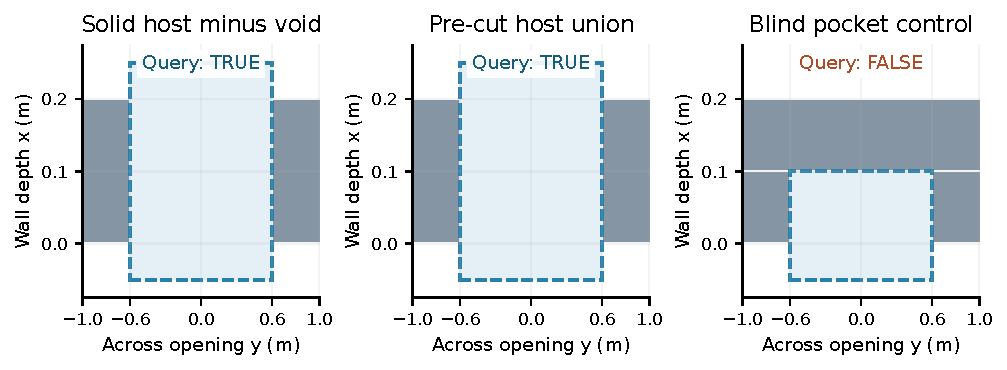
\includegraphics[width=\linewidth]{figures/verification/opening_encoding_equivalence.pdf}
\caption{Synthetic encoding-equivalence check at $z=1$ m. Gray is retained wall material; blue marks the declared void. The first two encodings yield the same material and connection verdict. The third is a true blind pocket and is rejected. Horizontal and vertical scales differ to expose the thin wall. These are software fixtures, not model outputs.}
\label{fig:opening-equivalence}
\end{figure}

The historical v1 study was generated under 2.2 and uniformly reassessed under 2.2.1 using the same retained raw outputs. Across its three routes, correct determinate readouts changed from 1,532/1,800 to 1,690/1,800: an increase of 158 measured readouts. This is a measurement correction, not improved model inference. Original outputs, original scores, and both evaluator versions remain preserved. The later N2 and CS1 cohorts prospectively use 2.2.1. The scorer checks input and evaluator freezes and compares raw-response hashes rather than selecting only favorable rescored cases.

\subsection{A remaining slab-encoding limitation}
The wall correction is not a proof of invariance for every host type. A later diagnostic examined ten preselected worlds whose issue sets were dominated by slab-opening handling. All ten transformations were attempted once. Eight preserved the occupied material and demonstrated label-sensitive geometric verdicts across ten slab-opening pairs. Two transformations changed the occupied material, so they do not establish an encoding false positive.

In the eight material-equivalent cases, the all-declared status changed from violation to unevaluable, not to pass: other unresolved checks remained. Fixed query readouts and registered statuses were unchanged in all ten attempts. The diagnostic produced no A/B all-declared pass gain and no new primary evaluator version. We therefore retain 2.2.1 primary scores and report this limitation instead of selectively substituting a more favorable encoding. The result also explains why a remaining violation count cannot automatically be read as the number of physically impossible buildings.

\subsection{Grounding, provenance, and what is not checked}
The source audit verifies whether the output names allowed sources, retains invalid active-source claims, and references existing declared entities. Given-point grounding uses exact source IDs and observation boxes, with an IoU threshold of 0.25 against approximate reference boxes. This is not camera-calibrated three-dimensional reconstruction, and source aliases are not silently normalized. A provenance edge is an inspectable declared dependency; it is not proof that a visual claim follows from its pixels. Evidence-revision experiments therefore score explicit knowledge, source status, dependencies, and retained readouts separately.

The implementation provides bounded constructive tests over rectilinear material and supported interfaces. It does not solve arbitrary three-dimensional satisfiability, certify load-bearing safety, enforce building codes, handle general meshes, or test a full human trajectory. Unknowns preserve these boundaries without counting as positive geometric success. These limits are part of the measured interface: the study tests whether models can construct and revise worlds inside that interface, while keeping answer correctness, material coherence, and visual grounding distinct.

\clearpage\section{Full GPT Results and Paired Analyses}\label{app:E}
\subsection{Allocation, configurations, and denominators}
The GPT record contains 688 allocated task stages: 288 v1 static tasks, 288 N2 static tasks, 48 CS1 static tasks, and 64 evidence-revision stages. The static total is therefore 624, not 688. Each static condition has R, A, and B. The eight recorded Codex configurations are 6 Astra, 6.1 Sol, 6.1 Terra, 6 Sol, 6 Luna, 5.6 Sol, 5.6 Terra, and 5.6 Luna, all with the recorded \texttt{xhigh} setting. These are eight product configurations from one provider family.

There are 684 standard-path raw files, of which 683 are nonempty. The frozen ledger classifies 651 stages as scored, seven as Schema failures, 25 as raw/parse failures, four as missing outputs, and one with a coarse output-limit label. The last label belongs to a CS1 \texttt{world:null} response and should not be read as a measured character overflow. The release retains the frozen status and this qualification. Appendix~\ref{app:J} reports failures separately from content errors.

Table~\ref{tab:E-main} uses every allocated determinate query opportunity. A failed output earns no correct readout but remains in the denominator. Table~\ref{tab:E-config} expands the result by configuration. The supplied B relations improve some constructions, but the improvement is neither universal nor sufficient to guarantee coherent geometry.

\begin{table}[htbp]\centering
\begin{tabular}{lrrr}\toprule Input & R & A & B\\\midrule
v1 & 599/600 & 541/600 & 550/600\\
N2 & 589/600 & 531/600 & 537/600\\
CS1 & 146/160 & 115/160 & 125/160\\\bottomrule
\end{tabular}
\caption{Correct determinate readouts under evaluator 2.2.1, including all allocated opportunities. v1 and N2 share buildings. CS1 B is 78.13\% under decimal half-up rounding.}\label{tab:E-main}
\end{table}

\begin{table}[htbp]\centering\small
\begin{tabular}{llrrrrr}
\toprule
Input & GPT config. & R & A & B & A valid & B valid \\
\midrule
v1 & 6 Astra & 75/75 & 71/75 & 75/75 & 12/12 & 12/12 \\
v1 & 6.1 Sol & 75/75 & 71/75 & 74/75 & 12/12 & 12/12 \\
v1 & 6.1 Terra & 75/75 & 68/75 & 74/75 & 11/12 & 12/12 \\
v1 & 6 Sol & 75/75 & 74/75 & 73/75 & 12/12 & 12/12 \\
v1 & 6 Luna & 74/75 & 63/75 & 63/75 & 11/12 & 11/12 \\
v1 & 5.6 Sol & 75/75 & 73/75 & 65/75 & 12/12 & 11/12 \\
v1 & 5.6 Terra & 75/75 & 66/75 & 61/75 & 11/12 & 10/12 \\
v1 & 5.6 Luna & 75/75 & 55/75 & 65/75 & 10/12 & 12/12 \\
N2 & 6 Astra & 74/75 & 63/75 & 69/75 & 11/12 & 11/12 \\
N2 & 6.1 Sol & 75/75 & 71/75 & 71/75 & 12/12 & 12/12 \\
N2 & 6.1 Terra & 74/75 & 75/75 & 75/75 & 12/12 & 12/12 \\
N2 & 6 Sol & 74/75 & 73/75 & 69/75 & 12/12 & 11/12 \\
N2 & 6 Luna & 72/75 & 55/75 & 69/75 & 10/12 & 12/12 \\
N2 & 5.6 Sol & 75/75 & 74/75 & 68/75 & 12/12 & 11/12 \\
N2 & 5.6 Terra & 72/75 & 53/75 & 58/75 & 10/12 & 10/12 \\
N2 & 5.6 Luna & 73/75 & 67/75 & 58/75 & 12/12 & 10/12 \\
CS1 & 6 Astra & 18/20 & 19/20 & 20/20 & 2/2 & 2/2 \\
CS1 & 6.1 Sol & 18/20 & 19/20 & 20/20 & 2/2 & 2/2 \\
CS1 & 6.1 Terra & 19/20 & 17/20 & 17/20 & 2/2 & 2/2 \\
CS1 & 6 Sol & 19/20 & 16/20 & 18/20 & 2/2 & 2/2 \\
CS1 & 6 Luna & 17/20 & 7/20 & 9/20 & 1/2 & 1/2 \\
CS1 & 5.6 Sol & 19/20 & 17/20 & 18/20 & 2/2 & 2/2 \\
CS1 & 5.6 Terra & 17/20 & 12/20 & 16/20 & 2/2 & 2/2 \\
CS1 & 5.6 Luna & 19/20 & 8/20 & 7/20 & 1/2 & 1/2 \\
\bottomrule
\end{tabular}

\caption{Full configuration results. v1/N2 each have 12 tasks per route, 75 determinate obligations per configuration; CS1 has two tasks and 20 obligations. A/B valid means contract-scorable, not geometrically correct.}\label{tab:E-config}
\end{table}

\subsection{A paired comparison on common-valid tasks}
The full denominator measures the delivered system, including format and delivery. To examine task-content differences, Table~\ref{tab:E-paired} pairs queries only when both compared outputs are contract-valid. It does not discard geometric errors. The resulting denominator can differ between R--A and A--B because validity depends on the compared routes.

\begin{table}[htbp]\centering\small
\begin{tabular}{llrrrrr}
\toprule
Input & Pair & $n$ & Both & First only & Second only & Neither \\
\midrule
N2 & R $\to$ A & 570 & 526 & 34 & 5 & 5 \\
N2 & A $\to$ B & 533 & 487 & 11 & 29 & 6 \\
CS1 & R $\to$ A & 140 & 113 & 15 & 2 & 10 \\
CS1 & A $\to$ B & 140 & 110 & 5 & 15 & 10 \\
\bottomrule
\end{tabular}

\caption{Common-valid paired outcomes. First-only means the first route is correct and the second is wrong or unevaluable. For R--A this is an answer-to-construction loss; for A--B, second-only is a relation-assisted rescue.}\label{tab:E-paired}
\end{table}

N2 has 34 R-correct/A-incorrect outcomes and five in the other direction among 570 common-valid obligations. The difference A minus R is $-5.09$ percentage points. A building-cluster bootstrap with 20,000 resamples and seed 20261105 gives a percentile interval of $[-9.29,-1.55]$ points. This interval describes the observed configuration ensemble on resampled buildings; it does not turn configurations or correlated questions into independent architectural samples.

For N2 A--B, B rescues 29 obligations and loses 11 among 533 common-valid pairs, a net difference of $+3.38$ points with interval $[0.19,6.42]$. Using all 600 allocated opportunities instead gives 50 rescues and 44 regressions, a net gain of six correct readouts. The two analyses answer different questions. The latter includes changes in output validity, while the former compares content on a shared valid subset. Neither should be substituted for the other without its denominator.

CS1 has 15 R-only versus two A-only outcomes, and 15 B-only versus five A-only outcomes, on 140 common-valid pairs for each contrast. Only two buildings contribute. We report these counts without a broad population confidence claim. The comparison is informative about these difficult drawings, but it is not a precise prevalence estimate for all complex staircases.

\subsection{Building and relation-type results}
Table~\ref{tab:E-building} shows the N2 and CS1 results by building, aggregated across the eight configurations. This aggregation keeps a hard building from disappearing in a high overall average. Table~\ref{tab:E-predicate} separates relation types. Both use full allocated opportunities; UNKNOWN is excluded from determinate accuracy and evaluated separately.

\begin{table}[htbp]\centering\small
\begin{tabular}{llrrr}
\toprule
Input & Building & R & A & B \\
\midrule
N2 & A01\_OCTAGON\_DC & 48/48 & 32/48 & 32/48 \\
N2 & A02\_DRAYTON & 45/48 & 45/48 & 48/48 \\
N2 & A06\_OCTAGON\_WI & 48/48 & 48/48 & 42/48 \\
N2 & B01\_nv0473 & 53/56 & 50/56 & 44/56 \\
N2 & B02\_mt0028 & 56/56 & 55/56 & 56/56 \\
N2 & B03\_az0061 & 47/48 & 44/48 & 48/48 \\
N2 & B04\_ca0801 & 39/40 & 36/40 & 39/40 \\
N2 & B05\_hi0032 & 48/48 & 36/48 & 37/48 \\
N2 & B06\_ga0030 & 48/48 & 48/48 & 48/48 \\
N2 & C01\_pr0070 & 48/48 & 42/48 & 36/48 \\
N2 & C02\_ut0027 & 46/48 & 41/48 & 47/48 \\
N2 & C03\_id0029 & 63/64 & 54/64 & 60/64 \\
CS1 & S01\_LOVELL\_HEALTH & 70/80 & 46/80 & 56/80 \\
CS1 & S02\_GAMBLE & 76/80 & 69/80 & 69/80 \\
\bottomrule
\end{tabular}

\caption{Correct readouts by building and route, pooling eight fixed configurations within each row. These are repeated measurements on a building, not independent buildings.}\label{tab:E-building}
\end{table}

\begin{table}[htbp]\centering\small
\begin{tabular}{llrrr}
\toprule
Input & Predicate & R & A & B \\
\midrule
N2 & above & 111/112 & 104/112 & 104/112 \\
N2 & connected\_by & 32/32 & 21/32 & 24/32 \\
N2 & disjoint & 56/56 & 54/56 & 53/56 \\
N2 & door\_host & 64/64 & 57/64 & 53/64 \\
N2 & identity\_assignment & 104/112 & 100/112 & 105/112 \\
N2 & same\_floor & 72/72 & 64/72 & 65/72 \\
N2 & stair\_connects & 15/16 & 12/16 & 11/16 \\
N2 & window\_host & 135/136 & 119/136 & 122/136 \\
CS1 & disjoint & 16/16 & 14/16 & 14/16 \\
CS1 & identity\_assignment & 59/64 & 49/64 & 56/64 \\
CS1 & same\_floor & 8/16 & 10/16 & 12/16 \\
CS1 & stair\_connects & 63/64 & 42/64 & 43/64 \\
\bottomrule
\end{tabular}

\caption{Determinate readouts by predicate. Differences combine relation difficulty, the available drawings, representation support, and delivery reliability.}\label{tab:E-predicate}
\end{table}

The granularity of a target can change the apparent error. Gamble Q01 is the ordinary \texttt{same\_floor} comparison, with R/A/B counts 8/8, 8/8, and 7/8. Gamble Q04 is a \texttt{stair\_connects} query, with 8/8, 4/8, and 2/8. Earlier narrative summaries incorrectly attached the ordinary-floor interpretation to Q04. The present tables use the frozen query IDs and predicates; no answer or score has been changed. Lovell Q04 is a separate local two-riser \texttt{same\_floor} question, with 0/8, 2/8, and 5/8. These examples show why a result must be traced to the actual query rather than to a remembered label.

\subsection{World coherence is a separate measurement}
Table~\ref{tab:E-world} adds geometry and coverage. All-relations-correct means that every determinate fixed query is correct for that world. Registered geometry checks the explicitly registered geometric roles and their dependencies. All-declared geometry also examines additional submitted entities. The joint result requires contract validity, required geometry coverage, correct determinate relations, and a PASS at the specified scope.

\begin{table}[htbp]\centering\small
\begin{tabular}{lrrrrrrr}
\toprule
Input & Alloc. & All rel. & Reg. & Joint reg. & Decl. & Joint decl. & Block \\
\midrule
v1/A & 96 & 77 & 46 & 43 & 9 & 9 & 5 \\
v1/B & 96 & 76 & 55 & 48 & 12 & 12 & 2 \\
N2/A & 96 & 69 & 50 & 42 & 16 & 14 & 1 \\
N2/B & 96 & 78 & 49 & 49 & 13 & 13 & 2 \\
CS1/A & 16 & 3 & 4 & 1 & 1 & 1 & 1 \\
CS1/B & 16 & 5 & 4 & 3 & 2 & 1 & 1 \\
\bottomrule
\end{tabular}

\caption{World-level results, out of allocated A/B worlds. Reg./Decl. are geometry PASS counts; joint also requires complete determinate correctness and coverage. Block means a definite represented material obstruction, a narrower class than all geometric violations.}\label{tab:E-world}
\end{table}

In N2, A has 69 all-relations-correct worlds and B has 78, but their all-declared joint counts are only 14 and 13 out of 96. A registered PASS is narrower: it does not certify every entity that the model chose to add. Conversely, an all-declared failure may concern a newly introduced fragment outside the registered geometric roles. This can be scientifically relevant without being a failure of a fixed local query.

N2 contains three definite material-blocking worlds. All three have every determinate fixed relation correct: 5.6 Luna's A and B Drayton Hall worlds, and its B Idaho City Schoolhouse world. In the latter, the internal staircase identity is itself queried by Q08, but its material geometry is outside the registered geometric-role list. It is therefore incorrect to call the internal stair wholly unqueried. The distinction is between an identity obligation and registered geometric scope.

\subsection{What the result establishes}
The observed configurations are generally strong at answering the selected relations, especially with semantic locators. Constructing a world imposes additional requirements that are not captured by a direct-answer score. Some losses are contract failures, some are interface or assembly errors, and a smaller set are explicit material conflicts. Relation assistance changes these outcomes but does not monotonically improve every building or every quality measure.

These results support measuring several output properties jointly. They do not establish a universal inability to reason spatially, a hidden internal world model, or a causal explanation based only on separate R/A generations. The casebook and common-valid analyses narrow the interpretation by identifying actual mechanisms and by retaining positive constructions as well as failures.

\clearpage\section{Cross-Family Qwen Experiment}\label{app:F}
\subsection{Actual model and request environment}
The cross-family comparison uses the requested and returned API snapshot \texttt{qwen3.8-max-0902}. The saved request enables thinking with a 32,768-token budget, sets maximum completion to 49,152 tokens, and uses temperature 0.6. The API returns ordinary text JSON. No forced repair, geometry feedback, or second primary attempt is applied.

Qwen receives the same public building images, locators, fixed questions, and A/B scientific contract. It runs as a tool-free multi-image request. Codex can instead read local assigned images and create crops from their pixels. Qwen R also receives a generic world Schema that is absent from the GPT R allowlist. The Schema contains no building-specific answers or reference coordinates. Nevertheless, the extra input and the tool difference are real conditions. The comparison is between model--interface systems, not a calibrated pure effect of neural weights or equal compute.

The request setting cannot be equated to Codex \texttt{xhigh}. A reasoning-token budget and a product effort label are different controls. Returned snapshot identifiers, request settings, usage where available, timing, and transport status are retained. A current provider model list would not establish what ran; the saved request and response records establish this experiment's identity.

\subsection{42 allocations, 39 complete replies, 38 scorable outputs}
The first two non-streaming submissions disconnect at about 61 seconds. They return no raw response or token usage and remain failed primary allocations. The remaining 40 are first submissions using a recorded streaming path. Six finish at concurrency two. The 34 not yet started are then queued at concurrency six; one streaming request also disconnects. Thus there are 42 allocated tasks, 39 complete replies, and 38 contract-scorable results. The incomplete allocations are not silently retried.

The transport has a 90-second socket-idle limit and checks a 900-second elapsed limit when a line arrives. This is not an exact 900-second process termination. A local scheduling error and the controlled queue change are recorded as execution events. They are not evidence of a spatial reasoning failure. The one completed Schema-invalid response is likewise distinct from the three transport losses.

\subsection{Full and common-valid results}
Table~\ref{tab:F-main} retains all allocated determinate opportunities. N2 yields 69/75 direct R answers, 62/75 A readouts, and 69/75 B readouts. Among valid outputs the corresponding counts are 69/69, 62/63, and 69/70. For CS1, all six task outputs are valid: R is 19/20, and both A and B are 16/20.

\begin{table}[htbp]\centering
\begin{tabular}{lrrr}
\toprule
Input & R & A & B \\
\midrule
N2 & 69/75 & 62/75 & 69/75 \\
CS1 & 19/20 & 16/20 & 16/20 \\
\bottomrule
\end{tabular}

\caption{Qwen full-denominator results under evaluator 2.2.1. The four invalid or absent task outputs are retained. CS1 has no such exclusion.}\label{tab:F-main}
\end{table}

\begin{table}[htbp]\centering\small
\begin{tabular}{llrrrrr}
\toprule
Input & Pair & $n$ & Both & First only & Second only & Neither \\
\midrule
N2 & R $\to$ A & 63 & 62 & 1 & 0 & 0 \\
N2 & A $\to$ B & 58 & 57 & 0 & 0 & 1 \\
CS1 & R $\to$ A & 20 & 16 & 3 & 0 & 1 \\
CS1 & A $\to$ B & 20 & 15 & 1 & 1 & 3 \\
\bottomrule
\end{tabular}

\caption{Qwen common-valid query pairs. These isolate shared valid outputs and should be read alongside the allocated denominator.}\label{tab:F-paired}
\end{table}

On the N2 R--A common-valid subset, 62 of 63 obligations are correct in both, and one is R-only. On the A--B subset, 57 of 58 are correct in both and one is wrong in both. There are no rescues or regressions in this shared valid A--B subset. The full 75-opportunity A--B comparison instead has 12 rescues and five regressions, a net gain of seven correct readouts. That gain is seven readouts, not seven percentage points, and it is largely tied to which task outputs are available and valid.

CS1 has 16 both-correct R--A pairs, three R-only pairs, no A-only pair, and one wrong in both. For A--B, 15 are correct in both, one is A-only, one B-only, and three wrong in both. B changes the identity of the errors without changing the total 16/20 score. This is why aggregate accuracy alone is inadequate for evaluating an assistance mechanism.

\subsection{Concrete construction losses}
All eight CS1 identity obligations are correct in each of R, A, and B for Qwen. The construction losses are therefore not explained by a blanket failure to associate the requested observations. Three R-correct/A-failed queries concern executable interfaces: Lovell Q09, Gamble Q04, and Gamble Q09.

Lovell Q09 has a submitted landing with \texttt{floor\_z}=5.29, while the top of its represented platform box is 5.79. The landing's declared floor is not its actual support surface. Gamble Q04 concerns a parent staircase whose submitted material does not match the union of its declared parts. Gamble Q09 names an endpoint as a corridor rather than supplying the required landing interface. These are three different contract/geometric mechanisms; they should not be collapsed into one visual detection error.

Lovell Q04 concerns a local two-riser transition. R and A are wrong, while B realizes that relation correctly. The B output also damages Q01's interface. This case supports both the usefulness and the limits of supplied relation values. A local rescue does not imply that the new world preserves other previously correct obligations.

There are 25 valid Qwen construction outputs and no definite material-blocking case in that set. This is a useful positive observation for the represented fragment. It does not erase interface violations or unknown coverage, and it does not establish that all true obstacles or full-building navigation were recovered.

\subsection{Grounding and source aliases}
Table~\ref{tab:F-boxes} separates exact requested-ID localization from a source-naming mismatch. The primary grounding parser expects observations linked to the requested view IDs. Some Qwen outputs use lexical aliases for the image source. Under a separate alias interpretation, 55 of 56 alias-linked boxes would meet IoU $\geq0.25$. That diagnostic is not inserted into the frozen primary score.

\begin{table}[htbp]\centering\small
\begin{tabular}{lrrrrrr}
\toprule
Input/route & $n$ & Pass & Low IoU & Alias & No box & Fail \\
\midrule
N2/A & 82 & 31 & 3 & 2 & 29 & 17 \\
N2/B & 82 & 8 & 2 & 48 & 18 & 6 \\
CS1/A & 11 & 0 & 0 & 4 & 7 & 0 \\
CS1/B & 11 & 2 & 0 & 2 & 7 & 0 \\
\bottomrule
\end{tabular}

\caption{Qwen given-point localization records: exact-ID pass, low IoU, source alias, no box, or failed allocation. Aliases are inspected separately instead of being silently rewritten into a pass.}\label{tab:F-boxes}
\end{table}

The large N2 B alias count means that a low strict grounding count cannot be interpreted directly as failure to see the target. It also does not prove correct physical identity: an overlapping box with a plausible source name still needs the correct object and instance binding. This diagnostic separates an interface explanation from the broader scientific grounding requirement.

\subsection{Scope of the cross-family conclusion}
The Qwen experiment adds one provider family and one snapshot condition. It shows strong relation answering, successful construction on many N2 obligations, and residual complex-staircase interface errors. It does not establish a family ranking across equal tools, independent repeats, or matched inference budgets. No Claude, Gemini, Grok, DeepSeek, or Seed results are claimed here because those experiments were not run in this record.

The next useful cross-family extension would preserve the same frozen core material while matching tool access or explicitly stratifying by interface. It should retain first outputs and transport failures, report both full and common-valid results, and add independently qualified buildings. Merely adding aliases from the same family would not answer the cross-family question.

\clearpage\section{Visual Grounding, Identity, and Uncertainty}\label{app:G}
\subsection{What the localization diagnostic measures}
The N2 task supplies a point at which to inspect an object and an optional class hint. Models then provide an image box and a physical-entity assignment. The reference boxes support a given-point localization diagnostic. They do not turn the experiment into automatic object detection: neither discovery recall over an entire drawing nor recovery of every room, opening, and stair is measured.

The primary overlap threshold is IoU $\geq0.25$. The criterion is relatively permissive and is reported with mean IoU and missing/unevaluable records. It measures approximate 2D extent around a specified target. It cannot by itself validate metric 3D placement, a host wall, a floor assignment, or cross-view physical identity. A model can put a reasonable box around an object while assigning it to the wrong instance.

\begin{table}[htbp]\centering
\begin{tabular}{llrrr}\toprule Input & Route & IoU gate & Mean IoU & Ref. NE\\\midrule
N2 & A & 446/656 & .491 & 16\\
N2 & B & 440/656 & .489 & 16\\
CS1 & A & 49/88 & .320 & 0\\
CS1 & B & 40/88 & .269 & 0\\\bottomrule
\end{tabular}
\caption{GPT localization, pooling the eight configurations. Ref. NE is reference-not-evaluable and is outside the listed IoU denominator. These are approximate image boxes at supplied points.}\label{tab:G-grounding}
\end{table}

Relation assistance does not improve these aggregate localization measures. N2 A/B mean IoU is almost unchanged, while CS1 B is lower. Correct relation values therefore do not substitute for locating the right image extent. The association is descriptive: A and B are independent generations, and the experiment does not isolate every possible localization mechanism.

\subsection{Observations, instances, and repeated labels}
An observation is a visible occurrence on a drawing; an entity is the physical instance that an observation may denote. Multiple observations can map to one entity. Two different windows can share a printed type code. A staircase assembly and one of its runs can overlap in an image without being the same semantic unit.

The executable reader's identity predicate compares submitted observation bindings. If two requested observations explicitly name the same entity, it reads SAME; unresolved bindings yield UNKNOWN. This is an inspectable output claim, not independent proof that the entity truly corresponds to the source building. Image-based qualification is still needed. The benchmark therefore reports identity readouts alongside grounding rather than treating either as a complete substitute for the other.

Figure~\ref{fig:G-identity} provides a source-linked identity example from Idaho City Schoolhouse. Its two crops correspond to O02 and O03 on different assigned pages. The frozen Q08 reference is TRUE. The audit links each crop to a public page and preserves its parent image hash. These human-review crops were not additional inputs during the model trials.

\begin{figure}[htbp]\centering
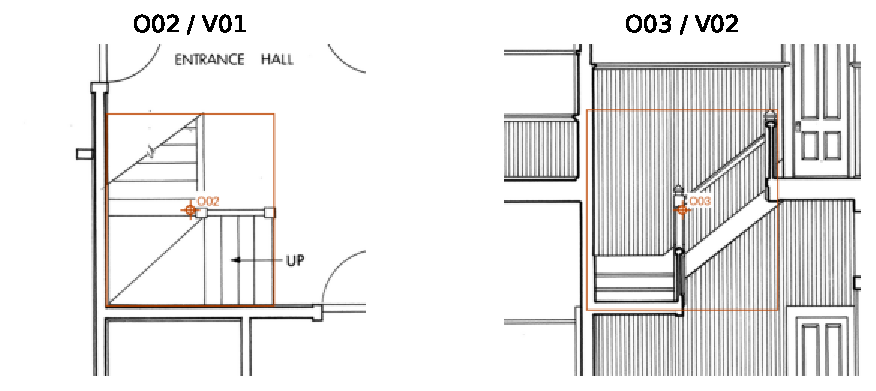
\includegraphics[width=.95\linewidth]{figures/identity_evidence.pdf}
\caption{Two drawing observations of the internal staircase in C03 (Q08). This is a reference-evidence panel, not a model detection. Image crops are shown for inspection; the package retains the complete pages. A correct identity binding does not by itself certify that the generated staircase is free of slab intrusion.}\label{fig:G-identity}
\end{figure}

\subsection{UNKNOWN as a supported result}
The unique unresolved identity concerns B04's cross-era observations. v1 returns the appropriate unresolved result in 18 of 24 allocations; N2 does so in only two of 24. The other 22 N2 outputs make unsupported definite assignments. Because the evidence does not establish a unique identity, these are failures of calibrated evidence use, not 22 independently proven physical mismatches.

Qwen R and A make definite SAME claims for this obligation. Its B task is missing because of the API service failure. These are two unsupported-certainty results and one unavailable result. The service failure is not reclassified as an identity decision. With only one uncertainty-bearing relation, the experiment cannot estimate a general calibration curve or uncertainty-detection accuracy across architecture.

\subsection{Source names and binding reliability}
A source identifier links a box or observation to its input image. An unrecognized alias can make the output hard to score even if the box is visually plausible. Appendix~\ref{app:F} reports the Qwen alias diagnostic separately. The same discipline applies to missing observations, duplicated entity IDs, and semantic target names: a convenient guessed mapping must not silently become reference truth.

The released records retain requested anchor IDs, source IDs, observation boxes, and entity bindings. This allows an auditor to distinguish at least four failures: no box at the requested point, a wrong extent, a source-ID mismatch, and a wrong physical binding despite a plausible box. The current aggregate score alone does not count all of these mechanisms independently; detailed cases must be inspected rather than inferred from the mean IoU.

The next grounding experiment should add more independently qualified same/different/unknown pairs and separate them from query wording. It should also test automatic candidate discovery without supplied points. Those are future measurements, not capabilities established by the current point-anchored record.

\clearpage\section{Evidence Revision and Historical Feedback Pilot}\label{app:H}
\subsection{Primary evidence-revision design}
A coherent world should respond to new evidence and later withdrawal without preserving unsupported facts or damaging unrelated supported relations. The retained revision experiment uses eight configurations on two buildings, with four stages per configuration--building pair. This gives 64 allocated stages. It is a small longitudinal experiment, separate from the N2 and CS1 static conditions.

E0 constructs a world from the initially permitted plans. A metric height that needs a section remains unknown. E1 adds the section evidence and asks for the resulting measured height. E2 withdraws that section and revises the world. F2 starts fresh with the same effective evidence available after the withdrawal. The E2--F2 comparison asks whether the incremental world agrees with a fresh construction under the same currently valid evidence.

The tasks retain source identifiers, support dependencies, explicit knowledge state, and selected unaffected relations. A successful E1 should incorporate the new supported height. A successful E2 should stop treating that measurement as known after its source is removed. It should also preserve supported spatial relations that do not depend on the withdrawn source.

The design tests submitted state, not hidden neural memory. Source withdrawal differs from assertion withdrawal, identity correction, and scope correction. Automatic raw-evidence recompilation for all four is not tested.

\subsection{Stage results with delivery retained}
Table~\ref{tab:H-stages} separates validity, explicit knowledge-state success, and relation preservation. The primary relation denominator is 80 per stage: five retained obligations for each of 16 allocations. The valid-only denominator is five times the valid allocation count. Reporting only valid outputs would conceal six E1 parse failures and other delivery losses.

\begin{table}[htbp]\centering\small
\begin{tabular}{lrrrrr}\toprule
Stage & Allocated & Valid & Knowledge & Relations/full & Relations/valid\\\midrule
E0 & 16 & 15 & 15/15 & 68/80 & 68/75\\
E1 & 16 & 10 & 10/10 & 49/80 & 49/50\\
E2 & 16 & 13 & 13/13 & 58/80 & 58/65\\
F2 & 16 & 14 & 14/14 & 65/80 & 65/70\\\bottomrule
\end{tabular}
\caption{Primary revision results. Knowledge success is conditional on a valid output. E1's ten valid worlds also realize the added height correctly. Relation denominators retain failed allocations in the full column.}\label{tab:H-stages}
\end{table}

E0 has one Schema failure. E1 has six raw/parse failures, E2 has three, and F2 has one raw/parse failure plus one missing output. Across the 52 valid stages, the explicit source-activity and active-dependency records are clean under the implemented checks. The ten valid E1 worlds also have the correct measured-height geometry. These are positive results for the submitted fields and bounded numeric obligation.

E2 and F2 are both valid for 11 configuration--building pairs. Their knowledge states agree in all 11, but only 51/55 retained relation readouts agree. E2 alone is wrong in three discordant obligations, and F2 alone in one. Clean metadata therefore does not guarantee identical world behavior.

The record establishes no incremental efficiency advantage. F2 is a new generation with a different prompt and history, not an equal-cost deterministic recomputation. Its differences from E2 may include stochastic construction and revision-history effects.

\subsection{Evidence can leak through a variable domain}
A previous American Farmhouse development diagnostic illustrates why deleting a support edge is insufficient. The recorded variable is the riser height in inches, not the floor-to-floor height used in the primary revision task. Its initial domain had been compiled using a later source as $D_h=\{7.5\}$ inches. Removing the explicit constraint $h=7.5$ leaves the variable domain unchanged. The feasible set still implies that height even though the supporting source is no longer active.

A proper evidence-independent initialization must instead retain the initially permissible domain $D_h^0$, and every active restriction must be derived from currently valid evidence. Candidate generation, identity bindings, cached factors, and precompiled domains all belong to the audit. This is ordinary dependency-management logic; the benchmark does not present it as a new truth-maintenance theorem~\cite{doyle1979}.

The primary model stages check explicit outputs and selected readouts. They do not provide a complete proof that all latent domain restrictions or earlier image interpretations have been recompiled from raw evidence. The distinction sets the boundary for the revision claim: the submitted knowledge state behaves well on valid stages, while relation preservation is imperfect and deeper recompilation remains to be measured.

\subsection{Historical A/B/C/D feedback pilot}
Before the 14-building study, an independent pilot used Robie House and Farnsworth House with eight configurations and four conditions, yielding 64 effective outputs. Its labels differ from the primary R/A/B design: A constructs directly; B receives correct relations; C revises the B seed once using actual checker feedback; D revises that same seed once after self-review. C and D do not regenerate a new B seed.

Under evaluator 2.1.0, the pilot has A/B/C/D relation totals 66/72, 66/72, 72/72, and 70/72. All-known-correct world counts are 14/16, 14/16, 16/16, and 14/16. These numbers are historical pilot results, not additional observations under evaluator 2.2.1 or independent new buildings in the primary study.

The apparent C gain requires mechanism inspection. Five restored readouts largely follow a repaired JSON comma; D also repairs the same syntax problem. Another C change corrects owner metadata rather than moving physical material. A headline such as ``feedback solves geometry'' would therefore be unsupported by the total score alone.

One 5.6 Terra B/C world still has a floor intruding into three stair treads. D removes that intrusion but loses a strict endpoint relation score. This example demonstrates why relation readout and material consistency need separate columns: an output can improve the represented material while becoming worse under an interface obligation.

The pilot also records 28 C/D outputs run under a wrong actual model condition. They were excluded for model-condition qualification and retained alongside the 64 effective outputs, giving 92 archived artifacts. They were not excluded because of their scores. The earlier two-building B0/B1 matrix is another pilot: 72/72 direct answers and 64/72 world readouts under evaluator 2.0, later 65/72 after an instrument correction. It is not pooled into the primary R/A/B totals.

\subsection{Revision conclusions and next test}
Valid stages satisfy the measured knowledge-state obligation, but revision does not always agree with fresh construction on retained relations. A stronger follow-up should freeze evidence-independent domains, add identity and scope corrections, and compare all bindings and geometric readouts with a fresh raw-input recompile. That study remains uncompleted.

\clearpage\section{Geometric Failure Casebook}
\label{app:I}

These seven cases separate evidence interpretation, executable representation,
geometric realization, and evaluator behavior. They are selected diagnostic
examples, not a random sample or an additional experiment cohort. Historical
development cases retain their original instruments; current N2 and CS1 cases
use frozen evaluator 2.2.1. We do not combine their scores or replace a failed
output with a repaired version. All drawings below show saved model coordinates
or an explicitly identified encoding diagnostic. No private residential
photographs are included. Machine-readable geometry extracts and the source
index identify each example as I1--I7.

\subsection{I1: a perimeter wall intersects both Loft stair flights}
\label{app:I1}

\textbf{Evidence.}
The exposed Loft development pilot combined drawings, images, and 18
historical topological statements. This case uses its recovered B1 world and saved
independent geometric witnesses, not a new N2 building. The response was
recorded as \texttt{TIMEOUT\_WITH\_RESPONSE}; recovering a complete artifact
does not turn that transport event into a normal completion.

\textbf{Output and computation.}
The two private stair runs occupy different $y$ channels. Their ninth treads
both end at $z=1.35$ in normalized model units. Two components of perimeter
wall \texttt{EL} extend to $z=2.8$ and cross these flights. The stored
raw-primitive and GEOS checks give an intersection volume of $0.03$ for
each specified tread and zero uncovered area across the blocked strip.

\textbf{Interpretation and reproduction.}
Correct stair identity and separated channels do not remove this material
conflict. The coordinates are hypothetical completions, not measurements of
the residence. Extract I1 expands the two original stair runs and intersects
them with the unchanged wall boxes; it contains no photograph.

\begin{figure}[htbp]
\centering
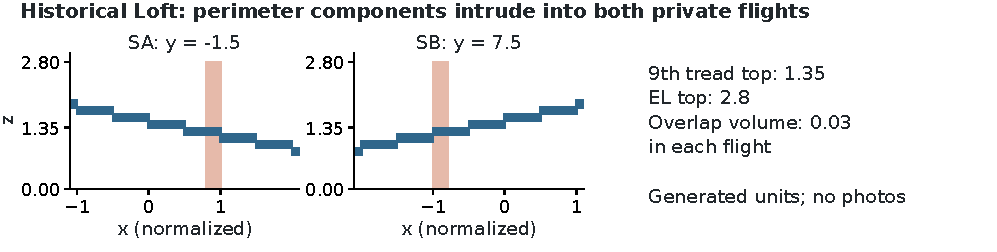
\includegraphics[width=.98\linewidth]{figures/casebook/I01_loft_wall_two_stairs.pdf}
\caption{Historical Loft geometry: the same declared perimeter has components
crossing both private flights. The panels use original normalized coordinates.}
\label{fig:I1-loft}
\end{figure}

\subsection{I2: a Farnsworth endpoint misses its declared upper terrace}
\label{app:I2}

\textbf{Evidence.}
The historical eight-configuration matrix evaluated Farnsworth House using
three measured-drawing pages. GPT-5.6 Luna answered its fixed geometric
questions correctly in B0, but its independent B1 world failed NF05 under
instrument 2.0.0.

\textbf{Output and computation.}
The generated upper terrace occupies $x\in[0,22]$ ft. The upper-flight endpoint
is $(31,-0.05,2.333\ldots)$ ft, and its landing is also near $x=31$.
Although endpoint and terrace-floor elevations agree, the endpoint lies
outside the terrace footprint. The saved proof reports that the upper endpoint
is not on its room floor; the lower endpoint passes that check.

\textbf{Interpretation and reproduction.}
This is a determinate geometric connection failure, rather than malformed
JSON. A connection label and an endpoint height do not establish incidence.
I2 retains the original endpoint, terrace, landing, and NF05 proof. The
historical result is not substituted into the current N2 table.

\begin{figure}[htbp]
\centering
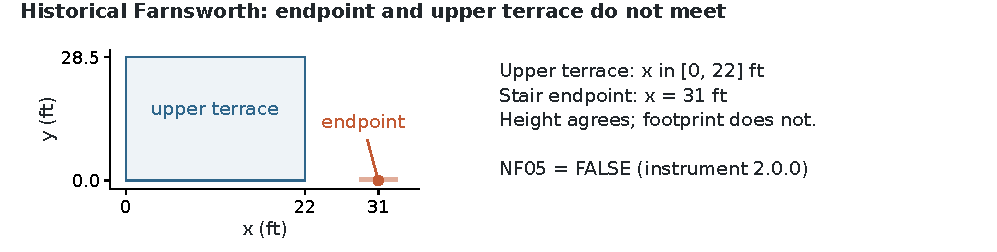
\includegraphics[width=.98\linewidth]{figures/casebook/I02_farnsworth_endpoint.pdf}
\caption{The generated endpoint and landing are laterally outside the
declared upper terrace. Equal height does not provide the missing contact.}
\label{fig:I2-endpoint}
\end{figure}

\subsection{I3: queried identity and unregistered material are different scopes}
\label{app:I3}

\textbf{Evidence.}
For Idaho City Schoolhouse, the N2 GPT-5.6 Luna B world satisfies all eight
fixed queries and passes registered geometry. Q08 correctly maps two
observations to \texttt{STAIR\_INTERNAL}. The exterior stair, not this
internal stair's material, belongs to the registered geometric obligations.

\textbf{Output and computation.}
The internal run rises from $(45,11,0)$ to $(45,17,10)$ ft in sixteen steps.
The uncut upper slab occupies $z\in[8,10]$ ft. The frozen material proof
identifies three tread surfaces at $8.125$, $8.750$, and $9.375$ ft,
covered across their full three-foot width.

\textbf{Interpretation and reproduction.}
Q08 checks the internal stair's identity, and that assignment is correct.
Its material is outside registered geometric scope but
inside all-declared scope. Extract I3 retains that scope list, Q08, and the
slab/run coordinates. Duplicate proof rows describe one physical conflict.

\begin{figure}[htbp]
\centering
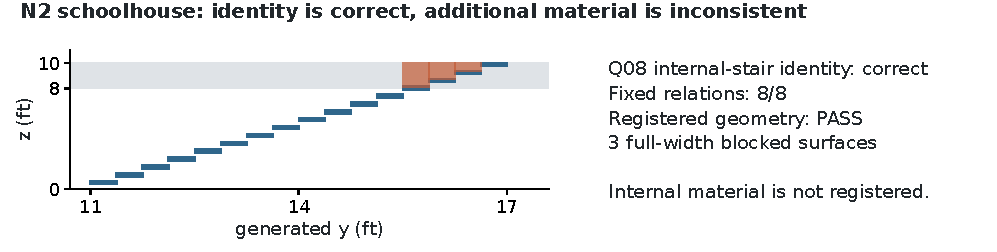
\includegraphics[width=.98\linewidth]{figures/casebook/I03_c03_registered_vs_material.pdf}
\caption{Identity is correct in Q08, while the internal-stair material is
inconsistent. Registered exterior-stair geometry remains a separate check.}
\label{fig:I3-scope}
\end{figure}

\subsection{I4: Lovell landing height is present but geometrically inconsistent}
\label{app:I4}

\textbf{Evidence.}
The CS1 Qwen model \texttt{qwen3.8-max-0902} produced a contract-valid
independent world for Lovell House. The fixed reference for Q09 requires
a staircase connection; evaluator 2.2.1 returns \texttt{UNKNOWN}.

\textbf{Output and computation.}
Landing \texttt{ld\_T03m} explicitly declares
\texttt{floor\_z=5.29} ft. Its box spans $z\in[5.29,5.79]$ ft.
The lower run also ends at $z=5.29$ ft. The floor field therefore agrees
with the material bottom rather than the supporting top. The saved reader
reports that the landing material and declared floor level are inconsistent.

\textbf{Interpretation and reproduction.}
This is not simply a missing-field error, nor evidence of a missing
visual detection. The available artifact localizes the failure to executable
support semantics. I4 compares the original landing box, floor field, run
endpoint, and Q09 proof without inserting a new platform or modifying a
height. Its unresolved readout remains distinct from a determinate false
connection.

\begin{figure}[htbp]
\centering
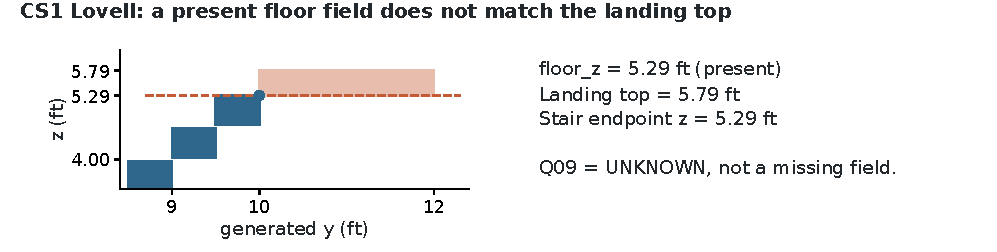
\includegraphics[width=.98\linewidth]{figures/casebook/I04_qwen_lovell_landing.pdf}
\caption{Lovell's generated landing floor is at its box bottom, 0.5 ft below
the material top. The field exists; its geometric meaning is inconsistent.}
\label{fig:I4-landing}
\end{figure}

\subsection{I5: a zero-thickness Astra landing violates the box contract}
\label{app:I5}

\textbf{Evidence.}
In the historical Farnsworth B1 artifact from GPT-6 Astra, NF05 is
\texttt{NOT\_EVALUABLE} under instrument 2.0.0. The JSON parses, but required
landing geometry is not executable.

\textbf{Output and computation.}
The upper-flight top interface has a positive rectangular footprint.
Both its minimum and maximum $z$ equal $2.333\ldots$ ft.
Consequently its box height is zero. The declared primitive requires
finite, strictly positive extent on all three axes; the compiler records
\texttt{INVALID\_GEOMETRY}.

\textbf{Interpretation and reproduction.}
A mathematical surface can be a reasonable intended interface while
violating this particular occupied-box representation. This observation
does not prove that the physical connection is impossible or that the
model reversed the building's levels. I5 preserves the zero-height box
and historical refusal. We do not thicken the interface or award a
counterfactual score.

\begin{figure}[htbp]
\centering
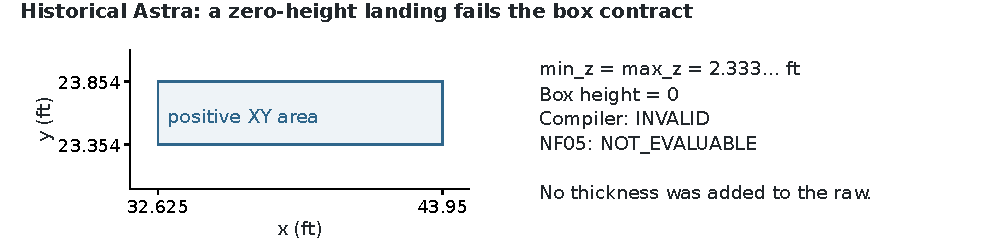
\includegraphics[width=.98\linewidth]{figures/casebook/I05_astra_zero_height.pdf}
\caption{Positive plan area does not satisfy a positive-volume box contract:
the original landing has exactly zero height.}
\label{fig:I5-contract}
\end{figure}

\subsection{I6: equivalent slab material triggers a different alarm}
\label{app:I6}

\textbf{Evidence.}
An existing diagnostic starts from Qwen's N2 Octagon House B output.
It changes only the slab's box encoding and retains the same opening.
This is a deterministic instrument diagnostic, not a new model response.

\textbf{Output and computation.}
Encoding one uses four pre-cut slab boxes; encoding two uses their envelope
with the same opening subtracted. The saved mutual-containment and difference
checks establish equal final material, with volume $155.489115$ ft$^3$.
Nevertheless, 2.2.1 reports one \texttt{DETACHED\_OPENING} row for the first
encoding and none for the second.

\textbf{Interpretation and reproduction.}
This establishes an encoding-sensitive instrument limitation, not a
physical obstruction. Four other violations remain unchanged; both full
verdicts are still \texttt{VIOLATION}. Fixed readouts and registered
geometry do not change. I6 retains both encodings, the unchanged void, and
the original equivalence proof; the diagnostic does not replace a primary
score.

\begin{figure}[htbp]
\centering
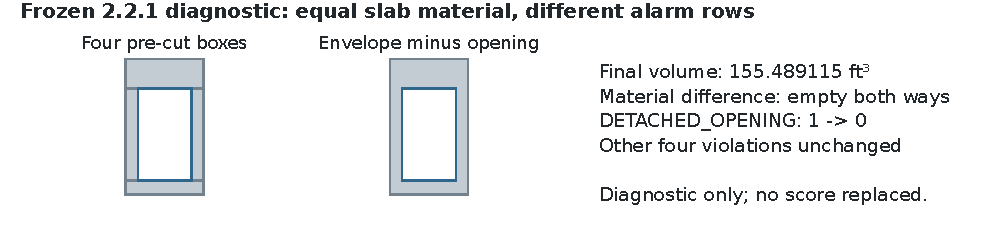
\includegraphics[width=.98\linewidth]{figures/casebook/I06_equivalent_slab_alarm.pdf}
\caption{Equal final slab material has different detached-opening alarm
counts. The diagnostic removes one alarm, not all remaining violations.}
\label{fig:I6-instrument}
\end{figure}

\subsection{I7: a genuine positive declared fragment}
\label{app:I7}

\textbf{Evidence.}
The N2 GPT-6.1 Terra A output for San Xavier del Bac provides a positive
control from the same frozen main-results collection, not a hand-built
reference or an \texttt{UNKNOWN} result.

\textbf{Output and computation.}
The world contains lower and upper tower spaces, a nave fragment, walls,
door and window openings, a font, and an upper support slab. All six fixed
relations are correct, all five target roles are present, registered
geometry passes, and verification is
\texttt{PASS\_DECLARED\_FRAGMENT}. The saved joint fragment-success flag is
true. The figure shows its actual hypothetical coordinate completion.

\textbf{Interpretation and reproduction.}
The benchmark admits successful worlds; failures are not required by its
definition. This positive applies to the bounded declaration and implemented
checks. It does not certify unseen parts of the mission or human navigation.
I7 reproduces the unchanged entity geometry, coverage record, query values,
and full-declaration verdict. The geometry and score are retained rather
than simplified into a synthetic ideal example.

\begin{figure}[htbp]
\centering
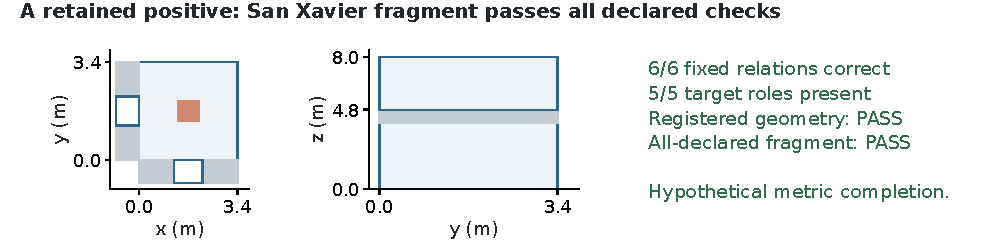
\includegraphics[width=.98\linewidth]{figures/casebook/I07_true_fragment_pass.pdf}
\caption{Tower detail of a real positive: six correct fixed relations, all five target
roles, and both registered and all-declared fragment checks pass.}
\label{fig:I7-positive}
\end{figure}

The supplied casebook verification script recomputes the numerical witnesses using only the Python standard library. Historical scores and unsupported semantic checks remain \texttt{NOT\_RECOMPUTED}.

\clearpage\section{Statistics, Failure Accounting, and Reproducibility}\label{app:J}
\subsection{Primary and conditional estimands}
Let $c_{mbqr}$ be one when configuration $m$ answers determinate query $q$ for building $b$ correctly in route $r$, and zero otherwise, including a failed or unevaluable allocated output. The primary accuracy is
\begin{equation}
\widehat a_r=\frac{\sum_{m,b,q\in Q_b^{\rm det}}c_{mbqr}}
{\sum_{m,b}|Q_b^{\rm det}|}.
\end{equation}
This is an allocated-opportunity measure. It includes delivery reliability and does not assign a cognitive cause to a failed parser result. UNKNOWN obligations are scored separately because evidence sufficiency differs from determinate truth.

For a route pair $(r,s)$, the common-valid subset contains the query opportunities for which both task outputs are contract-scorable. A paired table counts both correct, first-only, second-only, and neither. Geometry failures within a valid world remain in this subset. The conditional paired difference is
\begin{equation}
\widehat\Delta_{s-r}=\frac{n_{s\text{-only}}-n_{r\text{-only}}}{n_{\rm common}}.
\end{equation}
This quantity must be accompanied by the common-valid denominator. It is not interchangeable with the difference between two full-denominator accuracies when validity changes across routes.

World success adds further requirements. For each allocated construction, we report the conjunction of contract validity, required coverage, all determinate relations correct, and geometry PASS. Registered and all-declared geometry use different scopes. A NOT\_EVALUABLE result is not a PASS. A material-block flag is a narrower diagnostic than every kind of geometric violation, so it is also reported separately.

\subsection{Bootstrap and dependence}
The recorded N2 paired intervals use 20,000 building-cluster bootstrap resamples with seed 20261105. A resample draws 12 building IDs with replacement. It retains the configuration/query measurements belonging to each drawn building and recomputes the paired difference. The reported interval is the 2.5th--97.5th percentile range.

This preserves within-building dependence rather than treating every relation as an independent sample. The eight configurations are fixed conditions from one family, not eight random provider draws. The analyses were developed after inspecting results and are exploratory. There is no correction establishing a confirmatory family of many predicate-wise tests. The two-building CS1 counts are shown without a broad bootstrap generalization claim.

v1 and N2 use the same 12 buildings. Pooling them as independent architectural samples would overstate the data. Likewise, 688 stages are not 688 independent buildings. These counts are still useful for task-level reliability and mechanism analysis; the distinction is about the estimand and uncertainty, not a reason to discard the observations.

\subsection{Status ledger and operational departures}
Table~\ref{tab:J-status} preserves the frozen failure categories. Missing/empty files, parsing, Schema validation, unknown geometry, a typed interface violation, and a physical obstruction occur at different stages. A single aggregate error rate cannot locate their causes.

\begin{table}[htbp]\centering\small
\begin{tabular}{lllrrrrrr}
\toprule
Family & Input & Route & Alloc. & Scored & P & S & M & L \\
\midrule
GPT & v1 & R & 96 & 96 & 0 & 0 & 0 & 0 \\
GPT & v1 & A & 96 & 91 & 1 & 2 & 2 & 0 \\
GPT & v1 & B & 96 & 92 & 2 & 2 & 0 & 0 \\
GPT & N2 & R & 96 & 96 & 0 & 0 & 0 & 0 \\
GPT & N2 & A & 96 & 91 & 4 & 1 & 0 & 0 \\
GPT & N2 & B & 96 & 89 & 6 & 0 & 1 & 0 \\
GPT & CS1 & R & 16 & 16 & 0 & 0 & 0 & 0 \\
GPT & CS1 & A & 16 & 14 & 0 & 1 & 0 & 1 \\
GPT & CS1 & B & 16 & 14 & 2 & 0 & 0 & 0 \\
GPT & revision & E0 & 16 & 15 & 0 & 1 & 0 & 0 \\
GPT & revision & E1 & 16 & 10 & 6 & 0 & 0 & 0 \\
GPT & revision & E2 & 16 & 13 & 3 & 0 & 0 & 0 \\
GPT & revision & F2 & 16 & 14 & 1 & 0 & 1 & 0 \\
Qwen & N2 & R & 12 & 11 & 0 & 0 & 1 & 0 \\
Qwen & N2 & A & 12 & 10 & 0 & 1 & 1 & 0 \\
Qwen & N2 & B & 12 & 11 & 0 & 0 & 1 & 0 \\
Qwen & CS1 & R & 2 & 2 & 0 & 0 & 0 & 0 \\
Qwen & CS1 & A & 2 & 2 & 0 & 0 & 0 & 0 \\
Qwen & CS1 & B & 2 & 2 & 0 & 0 & 0 & 0 \\
\bottomrule
\end{tabular}

\caption{Frozen task statuses. P is raw/parse failure, S Schema failure, M missing output, and L the coarse limit label. The CS1 L case is a null world, not a measured size breach. Qwen M includes its three transport losses.}\label{tab:J-status}
\end{table}

Original outputs are not repaired. A uniquely retained artifact at a wrong location remains a diagnostic rather than a primary replacement. Complete host/session logs stay in the internal record because they can contain personal information. The anonymous package instead includes the task ledger, raw-output derivatives, model settings, source hashes, public input material, and the static scoring dependencies.

\subsection{What is actually replayable}
The package is organized around the chain
\begin{center}
saved response $\rightarrow$ strict parse $\rightarrow$ Schema validation $\rightarrow$\par
frozen bounded reader/compiler $\rightarrow$ per-query and world diagnostics.
\end{center}
It includes all 723 existing standard-path raw files as anonymous derivatives, and records seven absent allocations rather than inventing files for them. It includes the 42 public page PNGs, portable case/query/reference files, the frozen executable Schema, geometry code, static and revision scoring code, and manifests. It does not call a model or require an API credential.

The replay script is a portable path wrapper around the frozen scientific functions. Geometry and Schema content hashes are recorded. Where environment paths must change, the manifest records the transformation rather than claiming the entire host workflow is byte-identical. The wrapper reproduces the primary per-task scientific signature, including failures, query readouts, geometry states, and revision fields. It does not copy a final score table and call that rescoring.

The local verification executes two complete 730-allocation replays: one from the retained local original responses, one from the anonymous exported responses. The count is 688 GPT stages plus 42 Qwen allocations, including the seven absent files. It compares each scientific signature to its frozen historical result and compares the two replay sets. Detailed receipts and hashes are in the release. An unpacked copy is also exercised to check that scoring does not accidentally depend on the original absolute project path.

This verifies deterministic scoring of the saved material on the tested macOS environment. It does not regenerate model outputs, reproduce live Codex routing, prove another operating system has been tested, or recover a provider's unreported inference implementation. The vendor binary is specific to macOS arm64 and CPython 3.13. Other compatible POSIX environments need the pinned requirements and remain untested. The frozen worker uses POSIX resource controls; Windows requires a separate process-limit adapter and is not supported by this release.

\subsection{Anonymous derivatives and provenance}
Some original responses contain personal absolute paths in source or archival provenance fields. The local originals remain untouched. The anonymous export masks identifying string spans while preserving the length and encoded byte count relevant to the output-size rule. It does not reserialize JSON, repair malformed text, alter entity IDs, move coordinates, or change relation values. Exported and original hashes are both retained in the private provenance map; the public manifest identifies derivatives explicitly.

This distinction avoids two errors: presenting a sanitized artifact as an unchanged original, or leaking private paths merely to preserve an exact byte-for-byte public copy. Scoring invariance is checked through the actual frozen reader, not assumed from a text-diff inspection. Malformed originals stay malformed in the release.

The anonymous archive excludes internal absolute-path maps, original private photographs, session logs, credentials, account pages, and the author's local source-directory names. The source catalogue keeps public building names because they are task evidence, not author identity. Public source links document provenance; they do not substitute for contributed material that the reviewer must retrieve elsewhere.

\subsection{Reproduction procedure and outputs}
Start with the package README and run its manifest verification. Install the pinned small Python dependencies only if they are not already available. Then run the offline replay command from the unpacked package root. The runner writes new outputs to a fresh directory. It does not overwrite the frozen reference scores or raw responses. The comparison report should show no change in scientific signatures for the released primary allocations.

The release also includes the 4,416-row static query table, configuration/route aggregates, paired counts and bootstrap specification, the 688-stage GPT ledger, the 42-task Qwen ledger, source qualifications, and evaluator diagnostic summaries. These tables enable transparent aggregation; the raw replay provides the stronger check that their readouts can be regenerated.

Main-paper claims have an internal claim-to-evidence index. It maps each major result to a main page/table or figure, the relevant appendix, machine-readable fields, source paths, and hashes. This internal index can retain local provenance without putting private paths in the anonymous archive. It is an author audit aid, not a replacement for the inspectable evidence in the release.

\subsection{Interpretation and remaining coverage}
The report establishes a benchmark and empirical decomposition: direct answers, construction readouts, represented material coherence, localization, and revision behavior can differ. It does not presuppose that a complex new network is necessary. The useful next methods should address a verified residual mechanism under matched information, with ordinary constraint and provenance methods as strong baselines.

Remaining work includes unprompted object discovery, further uncertainty cases and building families, metric reconstruction, and raw-evidence recompilation after identity/scope changes. Appendix~\ref{app:D} records the checker's remaining material-encoding sensitivity.

\clearpage
\section*{LLM Usage}
\addcontentsline{toc}{section}{LLM Usage and References}
AI assistants supported code development, experiment organization, source-linked analysis, and manuscript drafting. The evaluated model outputs are retained as experimental records. The author reports personally checking all 96 reference relations. This confirmation is recorded separately from the original AI-assisted annotation metadata; it is not an independent expert certification. Deterministic compilation and rescoring do not count as new model trials.
\bibliographystyle{plainnat}
\bibliography{references}
\end{document}
